\documentclass[cheatsheet.tex]{subfiles}
\begin{document}
\textbf{features (aka attributes)} A mapping from the instance space X to the feature domain F. model can be thought of as just a new feature, particular combination of the input features, constructed to solve the task at hand. \textbf{Types} Quantitative(numeric scale, age), Ordinal(ordered set, ranks), Categorical(unordered set, color). \textbf{Statistics} Mode, Median, mean, range, std, Skewness, Kurtosis, Percentiles, Deciles, Quartiles, Interquartile range \textbf{Plots} histogram, Percentile plot(CDF, Shows cumulative fraction of data - what \% fall below a given value)
\\
\textbf{tree models} ignore the scale of quantitative features, treating them as ordinal.
\\
\textbf{Feature construction and selection} constructed new features from the given feature set, then select a suitable subset prior to learning(equal-frequency/width Discretisation, divisive/agglomerative discretisation, Thresholding, kernel methods, N-grams, Cartesian products of categorical features.)
\\
\textbf{kNN} \textbullet Classify a new instance by taking a vote of the $\geq1$ nearest exemplars. \textbullet vote among all neighbors within a fixed radius r \textbullet combine the two, stopping when $count > k$ or $dist. > r$ \textbullet distance weighting, the closer an exemplar is to the instance, the more its vote counts. \textbf{ties} Preference to the 1NN, or Random choice. 
\textbf{Pros} train $O(n)$, simple, intuitive 
\textbf{Cons} test $O(n)$ require a good deal of storage, and can't easily represent a specific boundary geometry, rely on a useful distance metric.
\\
\textbf{Clustering vs. classification} In a classifier, possible class labels are provided. In a clustering problem, possible labels are the cluster labels learned from the training set. \textbf{Assigning} of labels or clusters to data points is classification.
\\
\textbf{Clustering} find clusters (groupings) that are compact with respect to the distance metric. \textbf{Cons} disregards the shape of the clusters
\\
\textbf{Scatter Matrix} The scatter of X is defined as the trace of the scatter matrix.(The trace is the sum of the diagonal elements of a square matrix). 
\\
\textbf{Kmeans} is to find a partition that minimises the total within-cluster scatter. NP-complete, no efficient solution to find the optimal clustering (data partition). \textbf{K-means algorithm} heuristic algorithm, not optimal, converge to local optimal, works quite well in most cases. run several times (with a random starting point) and then the best solution is selected(the solution with the smallest within-cluster scatter). 
\\
\textbf{Kmedoids} medoid of a set of points is the point with the minimal average dissimilarity (distance) to all other points in the set. \textbf{partitioning around medoids (PAM)} that tries to improve a clustering locally by swapping medoids with other data points\\
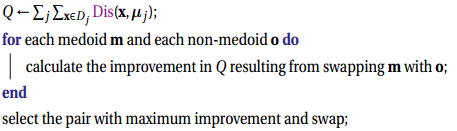
\includegraphics[width=.8\linewidth]{pam.png}
\\
\textbf{PCA} dimensionality reduction, finding the intrinsic linear structure in the data. eigenvalues can give clues to the inherent dimensionality of the data. 
\end{document}
